\RequirePackage{lineno}
\documentclass[aps,prl,reprint,twocolumn,groupedaddress,showpacs]{revtex4-1}
%\documentclass[aps,prl,reprint,twocolumn,groupedaddress,showpacs]{revtex4}
%\documentclass[10pt,reprint]{iopart}
%\documentclass[11pt]{article}
%\documentclass{pnastwo}
%\usepackage{color}
\usepackage[pdftex]{graphicx}
\usepackage{epstopdf}
\usepackage{bm}
\usepackage{amssymb}
\usepackage{psfrag}
\usepackage{color}
\usepackage{amsbsy}      
\usepackage{amsmath}
\usepackage{lineno}
\usepackage{natbib} 
\bibliographystyle{unsrt}
\usepackage{amsmath}
\graphicspath{{./figures/}}
%\usepackage{MnSymbol}


\newcommand{\bsigma}{{\boldsymbol\sigma}}
\def\alphaeff{\alpha_{\mathrm{eff}}}
\def\a{\alpha}
\def\b{{\bf b}}
\def\c{{\bf c}}
\def\d{{\bf d}}
\def\dd{\mbox{d}}
\def\dz{\delta z}
\def\ve{\varepsilon}
\def\eps{\epsilon}
\def\f{{\bf f}}
\def\g{\gamma}
\def\r{{\bf r}}
\def\rp{{\bf r}_{\perp}}
\def\q{{\bf q}}
\def\k{\kappa}
\def\u{{\bf u}}
\def\t{{\bf t}}
\def\w{{\bf w}}
\def\x{{\bf x}}
\def\y{{\bf y}}
\def\l{\ell}
\def\o{\omega}
\def\p{{\bf p}}
\def\s{\sigma}
\def\vp{\varphi}
\def\D{\Delta}
\def\F{{\bf F}}
\def\H{{\bf H}}
\def\K{{\bf K}}
\def\L{{\bf L}}
\def\Q{{\bf Q}}
\def\S{{\bf S}}
\def\T{{\bf T}}
\def\U{{\bf U}}
\def\V{{\bf V}}
\def\W{{\bf W}}  
\def\F{{\bf F}}                
\def\P{{\bf P}}
\def\Pt{\tilde{P}}
%\def\s{\mathbf{\sigma}}
\newcommand{\bs}{\boldsymbol{\sigma}}
\newcommand{\Conv}{\mathop{\scalebox{1.5}{\raisebox{-0.2ex}{$\ast$}}}}%

%\usepackage{fullpage}
\newcommand{\RR}{\mathbb{R}}


\begin{document}

\title{Reconstruction of localized force distributions in cells and tissues from substrate displacements using physically-consistent regularization}

%\author{Yanli Liu and Tom Chou} 
\affiliation{Depts. of
Biomathematics and Mathematics, UCLA, Los Angeles, CA 90095-1766}


%\maketitle 

%\begin{article}


%\runninglinenumbers*

\begin{abstract}
We develop a method to reconstruct, from measured displacements of the
underlying elastic substrate, the spatially dependent forces that
cells or tissues impart on them. Since these sources of force
typically arise from focal adhesions, with are localized or
``compact,'' and discontinuous, we solve this inverse problem using
methods of optimization useful for image segmentation. In addition to
the standard quadratic data mismatch terms (that defines least-squares
fitting), we motivate a term in in the objective function which
penalizes variations in the tensor invariants of the reconstructed stress while
preserving boundaries.   By minimizing
the objective function subject to physical constraints, we are able to
efficiently reconstruct stress fields with localized structure from
simulated and experimental substrate displacements. We provide a
numerical method for setting up a discretized inverse problem that that
 is solvable by standard convex optimization techniques. Our method incorporates
the exact solution of the forward problem accurate to first-order finite-difference approximation
in the stress tensor. For utility with newly-available high-resolution data, we motivate
the use of distance-based cutoffs for data inclusion and find under loose regularity
conditions the reconstruction error that results.
\end{abstract}
\maketitle

\section{Introduction}

Cell motility and response to signals have hitherto almost always been
studied in two-dimensional geometries in which cells are placed on a
flat elastic substrate.  Dynamic adhesion between the cells and the
substrate are realized through {\it e.g.}, lamellapodia, filapodia,
and dynamically reorganizing focal adhesions.  Such structures are
spatially localized, as shown in Fig.~\ref{FIG1}. Similarly, on larger
length scales, a collection of cells can give rise to localized stress
distributions. For example, the leading edge of a cell layer produces
the pulling force that leads to migration in wound healing assays.

\begin{figure}[t]
\begin{center}
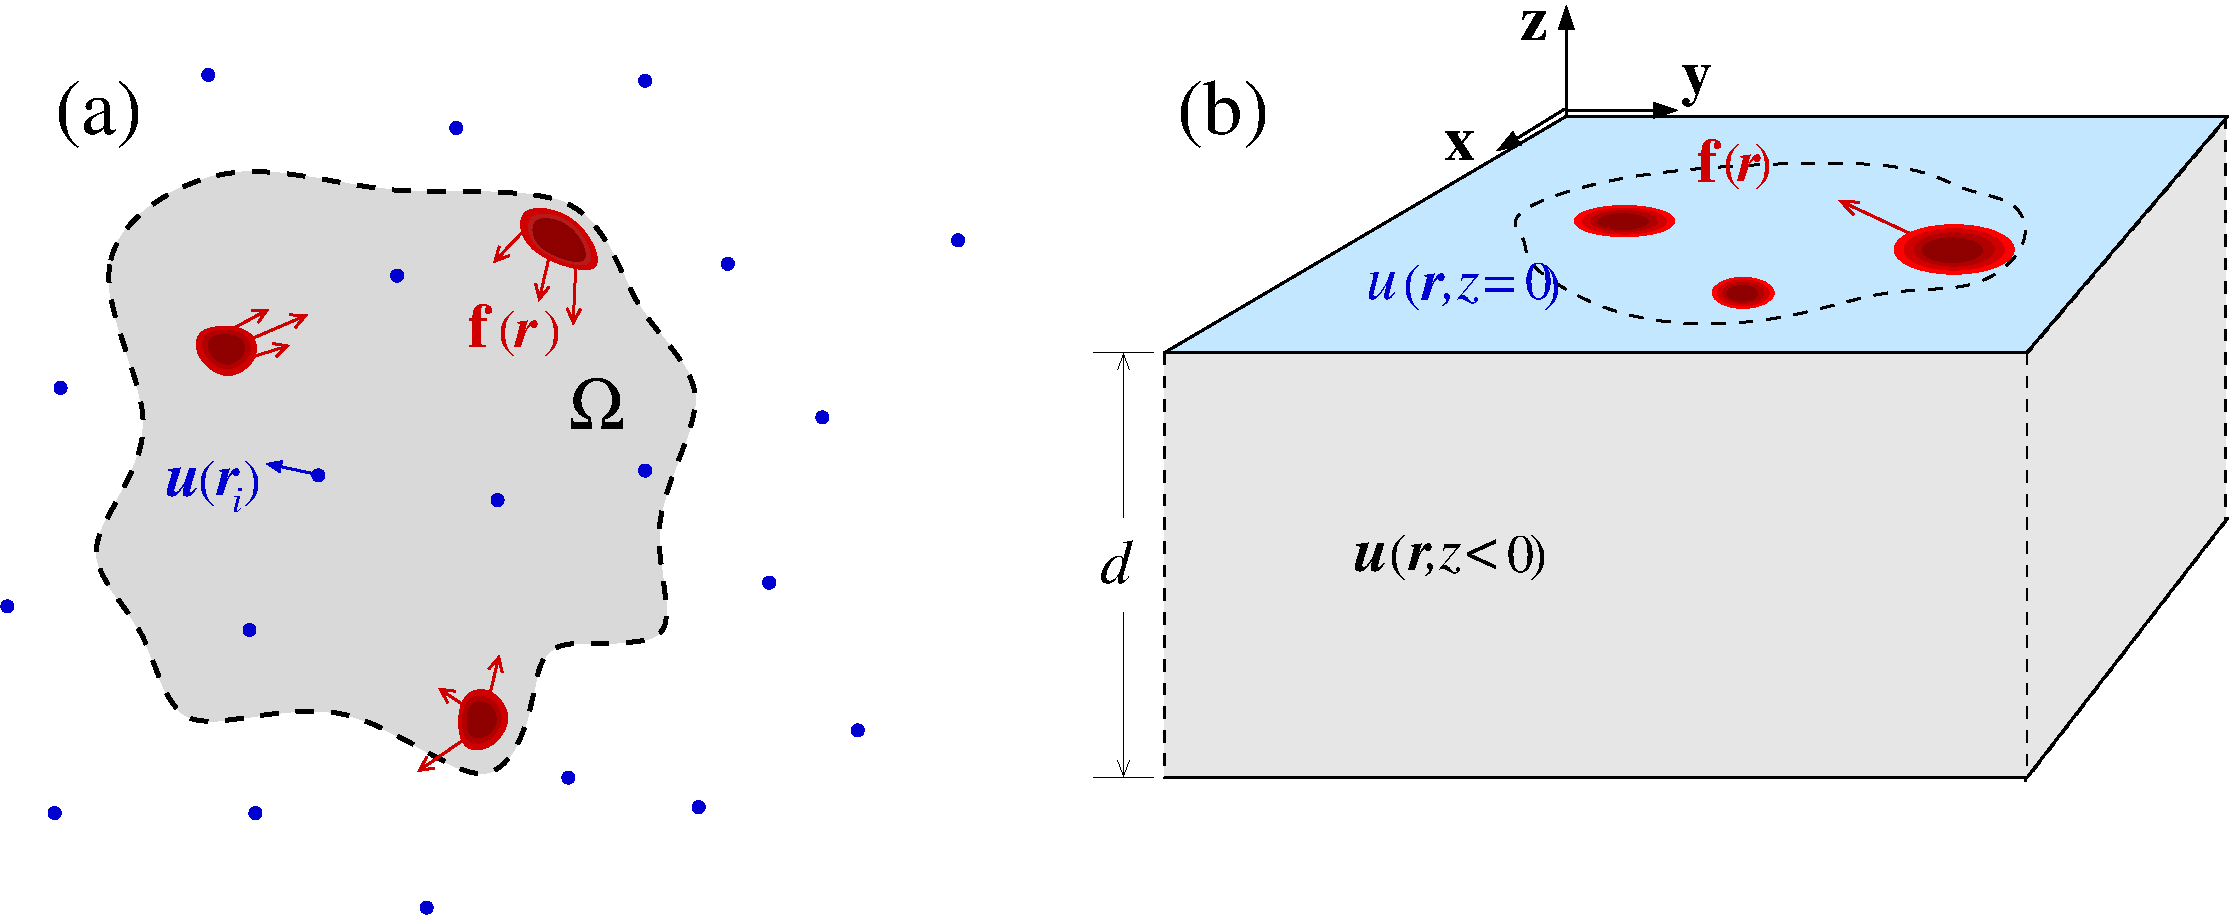
\includegraphics[width=\linewidth]{Fig1}
\caption{A schematic of an isolated cell. (a) The boundary of the cell
  footprint is denoted by the dashed curve, the stress field is
  represented by the red regions that impart a stress ${\bf F}(x,y)$
  on the surface. Displacements ${\bf u}(\r_{i})$ of the elastic
  medium are measured at position $\r_{i} =
  x_{i}\hat{x}+y_{i}\hat{y}+z_{i}\hat{z}$ (blue dots) that can be
  inside or outside the cell footprint, on the surface ($z_{i}=0$), or
  below the surface ($z_{i}<0$). (b). A perspective view of the
  elastic substrate and cellular footprint.}
\label{FIG1}
\end{center}
\end{figure}


Dynamically varying force generating structures are often small and
difficult to image, especially without biochemical modification such
as incorporation of fluorescent dyes. Therefore, other methods for
inferring their positions and magnitudes have been developed. The
simplest method relies on measuring the displacement of fiduciary
markers, such as gold nanoparticles, embedded in the elastic
substrate. The measured displacements are an indirect probe of the
force-generating structures.  Any inversion method should be able to
not only reconstruct the positions and magnitudes of the stress field,
but should ideally be able to capture potentially sharp boundaries of
the stress-generating structures.

Therefore, we develop a novel method for elastic stress source
recovery using ideas developed for image segmentation.  This class of
methods relies on optimization that uses an $L_{1}$ regularization
term in the objective function.  This type of regularization term is
not derived from a fundamental physical law, but represents a prior
knowledge that the function to be recovered is sparse in content
except near edges.  Nonetheless, our new objective will be constructed
to obey physical constraints and symmetries.

In the next section, we review the basic linear equations of
elasticity that describe the displacement field as a function of an
arbitrary surface stress distribution. This model is then used to
construct the data mismatch term in an objective function. We then
motivate regularization and constraint terms to construct the full
objective function. Finally, given simulated and experimental data, we
minimize our objective function using a modified split-Bregman
algorithm and reconstruct the given stress fields. Our method provides
good reconstruction of localized structures that exhibit desirable
qualities such as the suppression of Gibbs ringing phenomenon at the
boundaries of the stress structures.


\section{Elastic Model}

In this section, we explicitly describe the elastic green's function
associated with a point force applied to the surface of a
semi-infinite half-space, as shown in Fig.~\ref{FIG1}(b). The domain
of the elastic medium is ${\cal D}=\left\{(x,y,z)|x,y\in
R,z\leq0\right\}$. We assume that the elastic medium is infinite
in depth ($d\to \infty$) and lateral extent.

The Green's function 
\begin{equation}
{\bf G^0} = \left[ \begin{matrix} G^0_{xx}(x,y,z) & G^0_{xy}(x,y,z) & G^0_{xz}(x,y,z) \\
	G^0_{yx}(x,y,z) & G^0_{xy}(x,y,z) & G^0_{yz}(x,y,z) \\
	G^0_{zx}(x,y,z) & G^0_{zy}(x,y,z) & G^0_{zz}(x,y,z) 
 \end{matrix} \right]
\end{equation}
for linear isotropic elasticity theory 
in the half-space is given by its components
%
\begin{align}
\lefteqn{G^0_{ss}(x,y,z) = }\nonumber\\
&\frac{1+\nu}{2\pi E}\left[\frac{2(1-\nu)R_{\perp}-z}{R_{\perp}(R_{\perp}-z)} + 
\frac{[2R_{\perp}(\nu R_{\perp}-z)+z^{2}]s^{2}}{R_{\perp}^{3}(R_{\perp}-z)^{2}}\right],
\end{align}
%\begin{equation}
%G_{yy} =\frac{1+\nu}{2\pi E}\left[\frac{2(1-\nu)R_{\perp}-z}{R_{\perp}(R_{\perp}-z)}
%+\frac{[2R_{\perp}(\nu R_{\perp}-z)+z^{2}]y^{2}}{R_{\perp}^{3}(R_{\perp}-z)^{2}}\right],
%\end{equation}
\begin{equation}
G^0_{zz}(x,y,z) =\frac{1+\nu}{2\pi E}\left(\frac{2(1-\nu)}{R_{\perp}}+\frac{z^{2}}{R_{\perp}^{3}}\right),
\end{equation}
\begin{equation} 
G^0_{xy}(x,y,z) = G_{yx}=\frac{1+\nu}{2\pi E}\frac{[2R_{\perp}(\nu R_{\perp}-z)+z^{2}]xy}{R_{\perp}^{3}
(R_{\perp}-z)^{2}},
\end{equation}
\begin{equation}
G^0_{sz, zs}(x,y,z) =\frac{1+\nu}{2\pi E}\left(\frac{sz}{R_{\perp}^{3}}\pm\frac{(1-2\nu)s}{R_{\perp}
(R_{\perp}-z)}\right),
\end{equation}
%
where $s=x,y$  the equation with $\pm$ corresponds to $G^0_{sz}$ and $G^0_{zs}$, respectively, 
and $R_{\perp} \equiv \sqrt{x^{2} +y^{2}}$. The Young's modulus and Poisson ratio of the elastic substrate are denoted by 
$E$ and $\nu$, respectively.   
The displacement of a material point at $(x,y,z\leq 0)$ in the medium due
to a stress distribution ${\bf F}$ is simply the convolution
$\u(\r) \equiv [u_x \ u_y\  u_z]^\intercal = {\bf G^0}\Conv\F$.



%, while for a surface-localized force distribution, 
%$\F=(F_{x}(x,y,z=0),F_{y}(x,y,z=0),F_{z}(x,y,z=0))$ the displacement would be

%\begin{equation}
%\left[\begin{array}{c} u_{x}\\u_{y}\\u_{z}\end{array}\right]=
%\left[\begin{array}{ccc} G_{xx}&G_{xy}&G_{xz}\\G_{yx}&G_{yy}&G_{yz}\\G_{zx}&G_{zy}&G_{zz}
%\end{array}\right]
%\left[\begin{array}{c} F_{x}\\F_{y}\\F_{z}\end{array}\right]
%\end{equation}
%
%
%For a force distributation
%
%\begin{equation}
%\F=(F_{x}(x,y),F_{y}(x,y),F_{z}(x,y)) 
%\end{equation}
% 
%exerting on the surface of the medium,the displacement would be:

%\begin{equation}
%u_{i}(\r) = \int \dd \r_{\perp}'\dd z'
%G_{ij}(\r_{\perp}-\r_{\perp}',z-z')
%F_{j}(\r_{\perp}', z'),
%\label{UMODEL0}
%\end{equation}
% 
%where $\r = (\r_{\perp},z)$, $\r_{\perp}=x\hat{x} + y\hat{y}$ and
%$\r_{\perp}'= x'\hat{x} + y'\hat{y}$.  We will use this expression for
%the displacement as the model for the data term in the objective
%function for our inverse problem.

For our specific problem, we shall specialize the forces to surface
stresses $\sigma_{x,y}$ that act on the plane perpendicular to the
$\hat{z}$ axis. We define the in-plane stress distribution, at depth $z$, as
$\bs(x,y,z) = \sigma_{xz}(x,y,z)\hat{x} + \sigma_{yz}(x,y,z)\hat{y}$. 
The resulting surface-level displacement fields become

\begin{align}
u_{x}(x,y) &= \int_\Omega \dd x'\dd y'G_{xx}( x-x',y-y')\sigma_{xz}(x',y') \nonumber\\
&\qquad +  \int_\Omega \dd x'\dd y'G_{xy}( x-x',y-y')\sigma_{yz}(x',y') \label{eq:UMODEL1x}  \\
u_y(x,y) &= \int_\Omega \dd x'\dd y'G_{yx}( x-x',y-y')\sigma_{xz}(x',y') \nonumber\\
&\qquad +  \int_\Omega \dd x'\dd y'G_{yy}( x-x',y-y')\sigma_{yz}(x',y'),  \label{eq:UMODEL1y}  
\end{align}
where
\begin{equation}
G_{\cdot,\cdot}(x,y) = G^0_{\cdot,\cdot}(x,y,z=0),
\end{equation}
and by abuse of notation,
\begin{equation}
\sigma_{xz}(x,y) = \sigma_{xz}(x,y,z=0) \quad \sigma_{yz}(x,y) = \sigma_{yz}(x,y,z=0) .
\end{equation}
Note that tangential stresses can lead to displacement data in the normal direction.

%




\section{Setup of inverse problem}

Here, we develop an objective function for which the minimizing
solution provides a good approximation to the underlying stress
field, while preserving discontinuities.
 The first component is simply a quadratic data mismatch term
defined by the sum over the displacements measured at the $N$
measurement positions at $\r_{i}$:


\begin{equation}
\Phi_{\rm data}[\bs] = \sum_{i}^{N}\vert \u^{\rm
  data}(\r_{i})- \u(\r_i)\vert^{2}.
\end{equation}
%
Since $\u^{\rm data}(\r_{i})$ is given, and $\u(\r_{i})$, is given by
Eqs.~\ref{eq:UMODEL1x} and~\ref{eq:UMODEL1y}, this contribution to the objective function is a
functional over the surface-stress function $\bs(\r_{\perp})$.  For simplicity, we will assume that 
the data points are sampled over an uniform grid with coordinates given $\{ (x_j,y_k) : j\in[1,2,\ldots,J], k\in[1,2,\ldots,K] \}.$

In Eqs~\ref{eq:UMODEL1x} and~\ref{eq:UMODEL1y}, we have restricted the domain of integration to the extent of the cell, $\Omega$, to emphasize that  $\boldsymbol\sigma$ has compact support. As a consequence of compact support, for a fixed, discretized approximation of $\sigma_{xz},\sigma_{yz}$, the displacements can be obtained exactly by solving an equivalent system of linear equations of finite dimension.

Here we explicitely define this system of linear equations given a piecewise-affine approximation of the stress field. Let us consider the first-order approximation of $\sigma_{xz}$ and $\sigma_{yz}$ using central finite differences, for $x\in[x_j - \delta x/2, x_j+\delta x/2) \cap y\in[y_j-\delta y/2, y_j + \delta y /2)$,
\begin{align}
\lefteqn{\sigma_{xz}(x,y) =\sigma_{xz}(x_i , y_j)  }\nonumber \\
& \qquad+ (x-x_i)\frac{\sigma_{xz}(x_{i+1},y_j) -\sigma_{xz}(x_{i-1},y_j) }{2\delta x}  \nonumber\\
&\qquad + (y-y_j)\frac{\sigma_{xz}(x_i,y_{j+1}) - \sigma_{xz}(x_i,y_{j-1}) }{2\delta y} \nonumber\\
&\qquad + \mathcal{O}(\delta x)^2 + \mathcal{O}(\delta y)^2,\label{eq:sigma_affine}
\end{align}
where $i,j$ denotes a tuple of grid coordinates. In effect, we are performing sub-pixel interpolation of the stress where the stress is fully-determined by its values at the grid vertices.

Now we may rewrite Eq.~\ref{eq:UMODEL1x}, for instance, to solve for the displacement at a location $(x_n,y_m)$, by decomposing the integral into a sum of integrals over grid cells
%
\begin{widetext}
\begin{align}
 \lefteqn{u_x(x_n,y_m) =} \nonumber\\
 & \sum_{(x_j,y_k)\in\Omega} \Bigg\{ \Bigg[\sigma_{xz}(x_j,y_k)  - x_j\left(\frac{\sigma_{xz}(x_{j+1},y_k) - \sigma_{xz}(x_{j-1},y_k) }{2\delta x }    \right)    -y_k\left( \frac{\sigma_{xz}(x_j,y_{k+1}) -  \sigma_{xz}(x_j,y_{k-1}) }{2\delta y}\right) \Bigg]{ \langle G_{xx} \rangle}^{nmjk} \nonumber \\
&\quad+\left[ \frac{\sigma_{xz}(x_{j+1},y_k) -  \sigma_{xz}(x_{j-1},y_k) }{2\delta x}   \right]\langle x'G_{xx} \rangle^{nmjk} + \left[  \frac{\sigma_{xz}(x_j,y_{k+1}) - \sigma_{xz}(x_j,y_{k-1}) }{2\delta y} \right] \langle y'G_{xx} \rangle^{nmjk}\nonumber\\
&\quad+  \Bigg[\sigma_{yz}(x_j,y_k) -x_j\left(\frac{\sigma_{yz}(x_{j+1},y_k) - \sigma_{yz}(x_{j-1},y_k) }{2\delta x}    \right)    -y_k\left( \frac{\sigma_{yz}(x_j,y_{k+1}) - \sigma_{yz}(x_j,y_{k-1}) }{2\delta y}\right) \Bigg] \langle G_{xy} \rangle^{nmjk}\nonumber \\
&\qquad +\left[ \frac{\sigma_{yz}(x_{j+1},y_k) -  \sigma_{yz}(x_{j-1},y_k) }{2\delta x}   \right]  \int_{y_k-\delta y/2}^{y_k+\delta y/2}  \langle x'G_{xy} \rangle^{nmjk} + \left[  \frac{\sigma_{yz}(x_j,y_{k+1}) - \sigma_{yz}(x_j,y_{k-1}) }{2\delta y} \right] \langle y'G_{xy} \rangle^{nmjk} \Bigg\},
\label{eq:ux_decomposed}
\end{align}
\end{widetext}
where
\begin{align}
\lefteqn{\langle G_{st} \rangle^{nmjk} = }\nonumber\\
&\qquad    \int_{y_k-\delta y/2}^{y_k+\delta y/2} \int_{x_j-\delta x/2}^{x_j+\delta x/2} G_{st}(x_n-x',y_m-y') \dd x' \dd y' \label{eq:G_ave} \\
\lefteqn{\langle uG_{st} \rangle^{nmjk} =}  \nonumber\\
&\qquad  \int_{y_k-\delta y/2}^{y_k+\delta y/2} \int_{x_j-\delta x/2}^{x_j+\delta x/2} uG_{st}(x_n-x',y_m-y') \dd x' \dd y', \label{eq:G_ave2} 
\end{align}
except that at the edges where we use one-sided differences so that we are only differentiating within $\Omega$. Explicit 
closed-form expressions for the integrals represented in Eqs.~\ref{eq:G_ave} and~\ref{eq:G_ave2} are given in the Supplemental Materials. A similar expression can be found for solving for $u_y$ (not shown).

Regrouping terms, we can now define the linear system of equations for solving for $u_x$ at all grid points simultaneously,
\begin{equation}
u_x^{nm} = X^{nmjk}\sigma_{xz}(x_j,y_k) + Y^{nmjk}\sigma_{yz}(x_j,y_k),
\end{equation}
where summation is implied over each index tuple $(j,k)$, and the coefficient matrices are defined as
\begin{align}
\lefteqn{X^{nmjk} = \langle G_{xx} \rangle^{nmjk} -  \langle G_{xx} \rangle^{n,m,j-1,k}\frac{x_{j-1}}{2\delta x} } \nonumber\\
&\quad  + \langle G_{xx} \rangle^{n,m,j+1,k}\frac{x_{j+1}}{2\delta x} -  \langle G_{xx} \rangle^{n,m,j,k-1}\frac{y_{k-1}}{2\delta y}  \nonumber\\
&\quad + \langle G_{xx} \rangle^{n,m,j,k+1}\frac{y_{k+1}}{2\delta y} -\frac{\langle x'G_{xx} \rangle^{n,m,j-1,k}}{2\delta x}  \nonumber\\
&\quad +\frac{\langle x'G_{xx} \rangle^{n,m,j+1,k}}{2\delta x} - \frac{\langle y'G_{xx} \rangle^{n,m,j,k-1}}{2\delta y} \nonumber\\
&\quad+\frac{\langle y'G_{xx} \rangle^{n,m,j,k+1}}{2\delta y} 
\end{align}
\begin{align}
\lefteqn{ Y^{n,m,j,k} =  \langle G_{xy} \rangle^{nmjk} - \langle G_{xy} \rangle^{n,m,j-1,k}\frac{x_{j-1}}{2\delta x} } \nonumber\\
&\quad+\langle G_{xy} \rangle^{n,m,j+1,k}\frac{x_{j+1}}{2\delta x} - \langle G_{xy} \rangle^{n,m,j,k-1}\frac{y_{k-1}}{2\delta y} \nonumber\\
&\quad+\langle G_{xy} \rangle^{n,m,j,k+1}\frac{y_{k+1}}{2\delta y}  -\frac{\langle x'G_{xy} \rangle^{n,m,j-1,k}}{2\delta x} \nonumber \\
&\quad +\frac{\langle x'G_{xy} \rangle^{n,m,j+1,k}}{2\delta x} - \frac{\langle y'G_{xy} \rangle^{n,m,j,k-1}}{2\delta y} \nonumber\\
 &\quad+\frac{\langle y'G_{xy} \rangle^{n,m,j,k+1}}{2\delta y}.
\end{align}


From the equation-counting perspective, the system of equations is exactly determined given that one has at least as many measurement points as grid cells in the resolution that one wishes to reconstruct the stress field, provided that one is able to measure displacements in both principle directions. However, in line experiments this is not the case. Furthermore, even if one is able to measure both displacements, the problem may still be highly ill-conditioned since measurements are taken in the presence of noise at a given level of precision.

\subsection{Physical regularization}

So far, the construction of the surface stress, even at the discrete
resolution where measurements are available, is ill-conditioned. We 
regularize this problem, by forcing the reconstruction to obey some physically-relevant
characteristics of the surface stress. First, since we are assuming inertial
effects are negligible, we require that the net for is zero, or that
\begin{equation}
\int_\Omega\sigma_{xz}(x,y)\dd x \dd y= \int_\Omega\sigma_{yz}(x,y)\dd x \dd y = 0 .
\end{equation}
Likewise, we require that there is no net torque, or that
\begin{equation}
\int_\Omega\sigma_{yz}(x,y)x \dd x \dd y  = \int_\Omega\sigma_{xz}(x,y)y \dd x \dd y .
\end{equation}
 
 %
 Finally, we would like to impose regularity on the reconstructed fields while preserving first
 rotational invariance and second sharp interfaces. To this end we employ a variant of a penalty
 used often in image processing applications, where we wish to penalize the $L_1$ norm of the
 variation in the fields, or the total variation. To do this in such a manner that is consistent with
the philosophy that rotation of the data should not affect the result, we penalize the total variation
norm of the invariants of the stress tensor. In the case of two-dimensional tensors, of which the surface stress
is an example, the tensor invariants are the trace
\begin{equation}
\textrm{Tr}(\bsigma) = \sigma_{xz} + \sigma_{yz}
\end{equation}
and the determinant
\begin{equation}
\textrm{Det}(\bsigma) = \sigma_{xz} \sigma_{yz}.
\end{equation}
Any regularization penalty imposed on the reconstruction problem must be a function
of these invariants in order to maintain rotational invariance of the reconstructed stress tensor.

For this manuscript, we will use the trace, but we note that it may also be natural to use the
logarithm of the determinant, in analogy to the log-likelihood arising in multivariate linear regression
problems of unknown variance. We now write the convex regularization functional, $\Phi = ||\sigma_{xz} + \sigma_{yz}||_{TV} $ the total variation of the trace of the tensor,
%
\begin{equation}
\Phi =  \int_\Omega | \nabla(\sigma_{xz}(x',y') + \sigma_{yz}(x',y') | \dd x'\dd y'.
\end{equation}

The corresponding penalized optimization problem
\begin{equation}
\bsigma^\star \vert \lambda = \arg\min_{\bsigma} \left\{ \Phi_{\textrm{data}}[\bsigma] + \lambda\Phi[\bsigma] \right\},
\end{equation}
subject to the constraints mentioned above,
where $\lambda>0$ is a tunable parameter. This problem
 is linear and is solvable within standard optimization routines. In our implementation, we use a second-order  quadratic cone solver. 
\subsection{Cut-off}
To reduce the size of the system of equations...

\section{Results}

\subsection{Comparison of norms}
\section{summary and Conclusions}



%%%%%%%%%%%%%%%%%%%%%%%%%%%%%%%%%%%%%%%%%%%%%%%%%%%%%%%%%%%%%%%%%%%%%%%%
%%%%%%%%%%%%%%%%%%%%%%%%%%%%%%%%%%%%%%%%%%%%%%%%%%%%%%%%%%%%%%%%%%%%%%%%
\end{document}
%%%%%%%%%%%%%%%%%%%%%%%%%%%%%%%%%%%%%%%%%%%%%%%%%%%%%%%%%%%%%%%%%%%%%%%%
%%%%%%%%%%%%%%%%%%%%%%%%%%%%%%%%%%%%%%%%%%%%%%%%%%%%%%%%%%%%%%%%%%%%%%%%

